
	\section{角量和线量的关系}
	\subsection{相关线量和角量}
	以下是圆周运动中的相关线量和角量。
	
	线量：速度$\mathbf{v}$、加速度$\mathbf{a}$
	
	角量：角速度$\omega$、角加速度$\alpha$
	
	\subsection{线量和角量的关系}
	设圆的半径为$R$。
	
	\begin{figure}[h]
		\centering
		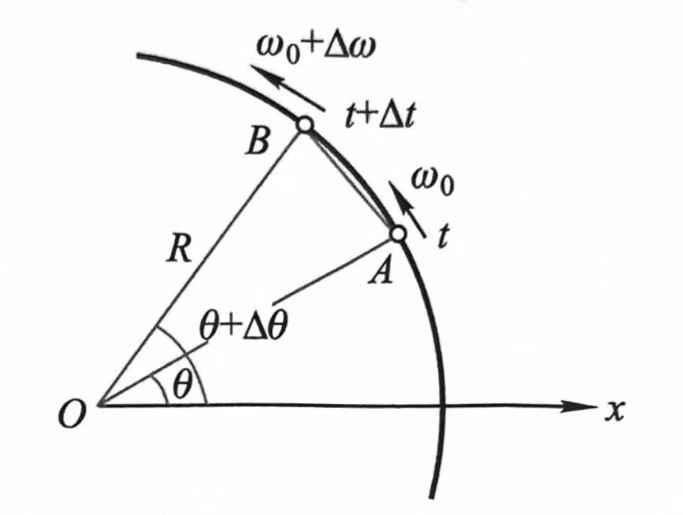
\includegraphics[width=0.5\textwidth]{images/ang-lin.jpg}
		\caption{线量和角量间的关系推导}
	\end{figure}
	
	\textbf{线速度和角速度：}
	\[
		v=R\omega
	\]
	
	\textbf{加速度和角加速度：}
	
	切向加速度
	\[
		a_t=R\alpha
	\]
	
	法向加速度
	\[
		a_n=\frac{v^2}{R}=v\omega=R\omega ^2
	\]
	
	\subsection{一般平面曲线运动中的加速度}
	质点沿轨迹作一般曲线运动时，上面讨论的有关变速圆周运动中加速度的结果也都是适用的。
	
	但法向加速度式中的R要用曲线在该点处的曲率半径$\rho$来代替。
	
	即
	\[
		\mathbf{a_t}=\frac{\mathrm{d}v}{\mathrm{d}t}\mathbf{e_t}
	\]
	\[
		\mathbf{a_n}=\frac{v^2}{\rho}\mathbf{e_n}
	\]
	\[
		\mathbf{a}=\mathbf{a_t}+\mathbf{a_n}=\frac{\mathrm{d}v}{\mathrm{d}t}\mathbf{e_t}+\frac{v^2}{\rho}\mathbf{e_n}
	\]
	
	法向加速度$a_n$处处指向曲率中心。 
	
	一般来说，曲线上各点的曲率中心和曲率半径是逐点变化的。
	
	\begin{figure}[h]
		\centering
		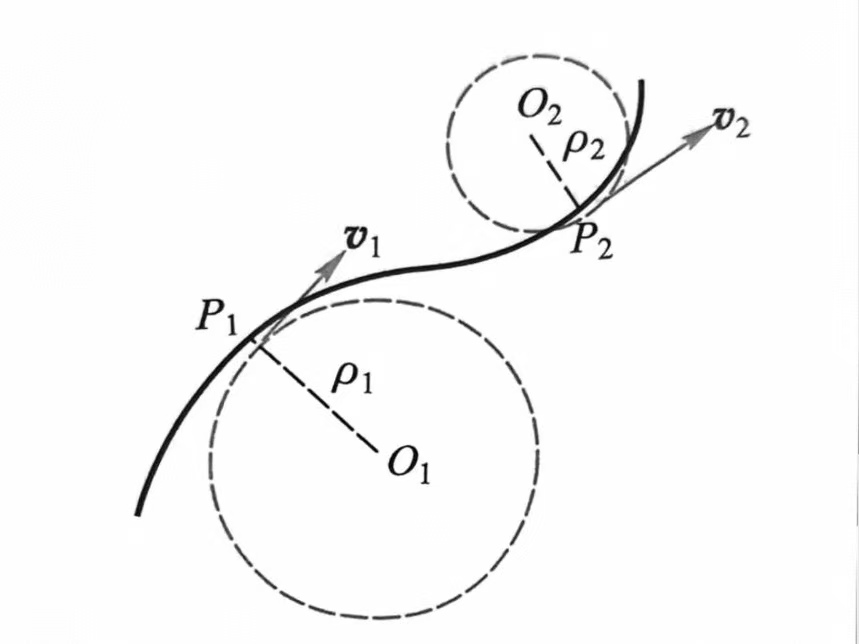
\includegraphics[width=0.5\textwidth]{images/rho.jpg}
		\caption{曲率圆和曲率半径}
	\end{figure}
